\begin{savequote}[45mm]
\ascii{Any fool can write code that a computer can understand. Good programmers write code that humans can understand.}
\qauthor{\ascii{- Martin Flower}}
\end{savequote}

\chapter{编程环境} 
\label{ch:prog-env}

\begin{content}

为了实现\tf{}的快速入门,本章将介绍\tf{}的编程环境,包括代码结构,工程构建,以便对\tf{}的系统架构建立基本的感性认识。

\end{content}

\section{代码结构}

\begin{content}

\subsection{克隆源码}

首先,从\ascii{Github}上克隆\tf{}的源代码。


\begin{leftbar}
\begin{python}
$ git clone git@github.com:tensorflow/tensorflow.git
\end{python}
\end{leftbar}

然后,切换到最新的稳定分支上。例如,\code{r1.4}分支。

\begin{leftbar}
\begin{python}
$ cd tensorflow
$ git checkout r1.4
\end{python}
\end{leftbar}

\subsection{源码结构}

运行如下命令,打印出\tf{}源码的组织结构。

\begin{leftbar}
\begin{python}[]
$ tree -d -L 1 ./tensorflow
\end{python}
\end{leftbar}

其中,本书将重点关注\code{core, python}组件,部分涉及\code{c, cc, stream\_executor}组件。

\begin{leftbar}
\begin{c++}[caption={TensorFlow源码结构}]
./tensorflow
├── c
├── cc
├── compiler
├── contrib
├── core
├── docs_src
├── examples
├── g3doc
├── go
├── java
├── python
├── stream_executor
├── tools
└── user_ops
\end{c++}
\end{leftbar}

截止当前最新发布的\ascii{1.4}版本,\tf{}代码库拥有大约\ascii{100}万代码。其中,包括\ascii{53}万行\ascii{C/C++}代码,\ascii{37}万行\ascii{Python}代码,而且代码规模在不断膨胀之中。其中,\ascii{Python}提供的\ascii{API}是最完善的;相比之下,其他编程语言的\ascii{API}尚未成熟,甚至处于起步阶段。

\begin{leftbar}
\begin{python}[caption={TensorFlow代码统计}]
-------------------------------------------------------
Language             files    blank    comment    code
-------------------------------------------------------
C++                   2238    77610     68275    443099
Python                1881    92018    151807    369399
C/C++ Header          1175    27392     46215     86691
Markdown               218     8859         2     30925
CMake                   50     2183       986     16398
Go                      28     1779     13290     15003
Java                    72     1789      3111      7779
Bourne Shell           103     1487      3105      6074
Protocol Buffers        87     1313      3339      3452
Objective C++            9      227       181      1201
C                        8      157       130       941
make                     4      105       136       612
XML                     25      135       265       315
Groovy                   3       46        74       246
Maven                    5       21         4       245
DOS Batch                9       30         0       143
Dockerfile               7       41        69       133
Perl                     2       29        38       130
Bourne Again Shell       3       24        63       111
JSON                     3        0         0        23
Objective C              1       10        13        21
YAML                     1        3        24        15
-------------------------------------------------------
SUM:                  5932   215258    291127    982956
-------------------------------------------------------
\end{python}
\end{leftbar}

\subsection{Core}

内核的源码结构如下所示,主要包括平台,实用函数库,基础框架,\ascii{Protobuf}定义,本地运行时,分布式运行时,图操作,\ascii{OP}定义,以及\ascii{Kernel}实现等组成,这是本书重点剖析的组件之一,将重点挖掘基础框架中隐藏的领域模型,追踪整个运行时环境的生命周期和图操作的详细过程,并揭示常见\ascii{OP}的\ascii{Kernel}实现原理和运行机制。

\begin{leftbar}
\begin{c++}[caption={Core源码结构}]
./tensorflow/core
├── common_runtime
├── debug
├── distributed_runtime
├── example
├── framework
├── graph
├── grappler
├── kernels
├── lib
├── ops
├── platform
├── profiler
├── protobuf
├── public
├── user_ops
└── util
\end{c++}
\end{leftbar}

其中,\code{core}主要由\code{C++}实现,大约拥有\ascii{26}万行代码。

\begin{leftbar}
\begin{python}[caption={Core代码统计}]
-------------------------------------------------------
Language             files    blank   comment      code
-------------------------------------------------------
C++                   1368    44791     38968    259289
C/C++ Header           653    15040     24474     50506
Protocol Buffers        57      736      2371      1806
Markdown                11      327         0      1285
JSON                     2        0         0        18
-------------------------------------------------------
SUM:                  2091    60894     65813    312904
-------------------------------------------------------
\end{python}
\end{leftbar}

\subsection{Python}

\ascii{Python}定义和实现了\tf{}的编程模型,并对外开放\ascii{API}供程序员使用,其源码结构如下所示,这也是本书重点剖析的部分。

\begin{leftbar}
\begin{c++}[caption={Python源码结构}]
./tensorflow/python
├── client
├── debug
├── estimator
├── feature_column
├── framework
├── grappler
├── kernel_tests
├── layers
├── lib
├── ops
├── platform
├── profiler
├── saved_model
├── summary
├── tools
├── training
├── user_ops
└── util
\end{c++}
\end{leftbar}

其中,该组件由\code{Python}实现,大约有\ascii{18}万行代码。

\begin{leftbar}
\begin{python}[caption={Python代码统计}]
-------------------------------------------------------
Language            files     blank   comment      code
-------------------------------------------------------
Python                714     45769     69407    179565
C++                    20       496       506      3658
C/C++ Header           15       207       387       363
Markdown                4        48         0       200
Protocol Buffers        3        16        10        71
Bourne Shell            1        13        28        68
-------------------------------------------------------
SUM:                  757     46549     70338    183925
-------------------------------------------------------
\end{python}
\end{leftbar}

\subsection{Contrib}

\code{contrib}是第三方贡献的编程库,它也是\tf{}标准化之前的实验性编程接口,犹如\ascii{Boost}社区与\ascii{C++}标准之间的关系。当\code{contrib}的接口成熟后,便会被\tf{}标准化,并从\code{contrib}中搬迁至\code{core, python}中,并正式对外发布。

\begin{leftbar}
\begin{python}[caption={Contrib源码结构}]
./tensorflow/contrib
├── android
├── batching
├── bayesflow
├── benchmark_tools
├── boosted_trees
├── cloud
├── cluster_resolver
├── cmake
├── compiler
├── copy_graph
├── crf
├── cudnn_rnn
├── data
├── decision_trees
├── deprecated
├── distributions
├── eager
├── factorization
├── ffmpeg
├── framework
├── fused_conv
├── gdr
├── graph_editor
├── grid_rnn
├── hooks
├── hvx
├── image
├── imperative
├── input_pipeline
├── integrate
├── keras
├── kernel_methods
├── labeled_tensor
├── layers
├── learn
├── legacy_seq2seq
├── linalg
├── linear_optimizer
├── lookup
├── losses
├── makefile
├── memory_stats
├── meta_graph_transform
├── metrics
├── mpi
├── nccl
├── ndlstm
├── nearest_neighbor
├── nn
├── opt
├── pi_examples
├── predictor
├── quantization
├── reduce_slice_ops
├── remote_fused_graph
├── resampler
├── rnn
├── saved_model
├── seq2seq
├── session_bundle
├── signal
├── slim
├── solvers
├── sparsemax
├── specs
├── staging
├── stat_summarizer
├── stateless
├── tensor_forest
├── tensorboard
├── testing
├── text
├── tfprof
├── timeseries
├── tpu
├── training
├── util
├── verbs
└── xla_tf_graph
\end{python}
\end{leftbar}

由于\tf{}社区相当活跃,\code{contrib}的变更相当频繁,截止\ascii{1.4}版本,大约有\ascii{23}万行代码,主要由\ascii{Python}设计和实现的编程接口,部分运行时由\ascii{C++}实现。

\begin{leftbar}
\begin{python}[caption={Contrib代码统计}]
-------------------------------------------------------
Language            files     blank   comment      code
-------------------------------------------------------
Python               1007     41436     75096    170355
C++                   201      5500      5313     32944
CMake                  48      2172       955     16358
C/C++ Header           99      1875      2867      6583
Markdown               46      1108         0      3485
Bourne Shell           18       232       386      1272
C                       7       151       118       931
Protocol Buffers       20       224       454       680
make                    4       105       136       612
Java                    2        77       209       335
Groovy                  1        10        20        75
Bourne Again Shell      1         6        15        59
Dockerfile              1         2         1        14
XML                     2         3         0         9
-------------------------------------------------------
SUM:                 1457     52901     85570    233712
-------------------------------------------------------
\end{python}
\end{leftbar}

\subsection{StreamExecutor}

\ascii{StreamExecutor}是\ascii{Google}另一个开源组件库,它提供了主机端(\ascii{host-side})的编程模型和运行时环境,实现了\ascii{CUDA}和\ascii{OpenCL}的统一封装。使得在主机端的代码中,可以将\ascii{Kernel}函数无缝地部署在\code{CUDA}或\code{OpenCL}的计算设备上执行。

目前,\ascii{StreamExecutor}被大量应用于\ascii{Google}内部\ascii{GPGPU}应用程序的运行时。其中,\tf{}运行时也包含了一个\ascii{StreamExecutor}的快照版本,用于封装\ascii{CUDA}和\code{OpenCL}的运行时。本书将简单介绍\ascii{CUDA}的编程模型和线程模型,并详细介绍\ascii{StreamExecutor}的系统架构与工作原理,揭示\ascii{Kernel}函数的实现模式和习惯用法。

\begin{leftbar}
\begin{c++}[caption={StreamExecutor源码结构}]
./tensorflow/stream_executor
├── cuda
├── host
├── lib
└── platform
\end{c++}
\end{leftbar}

其中,\ascii{StreamExecutor}使用\code{C++}实现,大约有\ascii{2.5}万行代码。

\begin{leftbar}
\begin{python}[caption={StreamExecutor代码统计}]
-------------------------------------------------------
Language            files     blank   comment      code
-------------------------------------------------------
C++                    43      2440      1196     16577
C/C++ Header           81      2322      5080      8625
-------------------------------------------------------
SUM:                  124      4762      6276     25202
-------------------------------------------------------
\end{python}
\end{leftbar}

\subsection{Compiler}

众所周知,灵活性是\tf{}最重要的设计目标和核心优势,因此\tf{}的系统架构具有良好的可扩展性。\tf{}可用于定义任意图结构,并使用异构的计算设备有效地执行。但是,熊掌与鱼翅不可兼得,当低级\ascii{OP}组合为计算子图时,并期望在\ascii{GPU}上有效执行时,运行时将启动更多的\ascii{Kernel}的运算。

因此,\tf{}分解和组合\ascii{OP}的方法,在运行时并不能保证以最有效的方式运行。此时,\ascii{XLA}技术孕育而生,它使用\ascii{JIT}编译技术来分析运行时的计算图,它将多个\ascii{OP}融合在一起,并生成更高效的本地机器代码,提升计算图的执行效率。

\begin{leftbar}
\begin{python}[caption={Compiler源码结构}]
./tensorflow/compiler
├── aot
├── jit
├── plugin
├── tests
├── tf2xla
└── xla
\end{python}
\end{leftbar}

\ascii{XLA}技术目前处于初级的研发阶段,是\tf{}社区较为活跃研究方向,截止目前代码规模大约为\ascii{12.5}万行,主要使用\ascii{C++}实现。

\begin{leftbar}
\begin{python}[caption={Compiler代码统计}]
-------------------------------------------------------
Language            files     blank   comment      code
-------------------------------------------------------
C++                   455     19010     18334    102537
C/C++ Header          250      5939     10323     15510
Python                 37      1255      1416      6446
Protocol Buffers        5       312       501       781
Markdown                2         0         0         3
-------------------------------------------------------
SUM:                  749     26516     30574    125277
-------------------------------------------------------
\end{python}
\end{leftbar}

\end{content}

\section{工程构建}

\begin{content}

在开始之前,尝试\tf{}源码的构建过程,了解\tf{}的基本构建方式、工具,及其依赖的组件库、第三方工具包,对于理解\tf{}工作原理具有很大的帮助。但是,因篇幅受限,本章仅以\ascii{Mac OS}系统为例,讲述\tf{}的源码编译、安装、及其验证过程。其他操作系统,请查阅\tf{}发布的官方文档。

\subsection{环境准备}

\ascii{TensorFlow}的前端是一个支持多语言的编程接口。因此,编译\ascii{TensorFlow}源代码之前,需要事先安装相关的编译器、解释器、及其运行时环境。例如,使用\ascii{Python}作为编程接口,需要事先安装\ascii{Python}解释器。其次,在构建系统之前,也需要事先安装\ascii{GCC}或\ascii{Clang}等\ascii{C++}编译器,用于编译后端系统实现。因为\ascii{TensorFlow}使用\ascii{C++11}语法实现,所以要保证安装\ascii{C++}编译器要支持\ascii{C++11}。另外,\ascii{TensorFlow}使用\ascii{Bazel}的构建工具,可以将其视为更高抽象的\ascii{Make}工具。不幸的是,\ascii{Bazel}使用\ascii{Java8}实现,其依赖于\ascii{JDK}。因此在安装\ascii{Bazel}之前,还得需要事先安装\ascii{1.8}及以上版本的\ascii{JDK}。

\subsubsection{安装JDK}

推荐从\ascii{Oracle}官网上下载\ascii{1.8}版本的\ascii{JDK},然后创建相关的环境变量,并将其添加到\code{~/.bashrc}的配置文件中。

\begin{leftbar}
\begin{python}
$ echo 'export JAVA_HOME=$(/usr/libexec/java_home)' >> ~/.bashrc
$ echo 'export PATH="$JAVA_HOME/bin:$PATH"' >> ~/.bashrc
\end{python}
\end{leftbar}

\subsubsection{安装Bazel}

在\ascii{Mac OS}上,可以使用\ascii{brew}安装\ascii{Bazel}。

\begin{leftbar}
\begin{python}
$ brew install bazel
\end{python}
\end{leftbar}

如果系统未安装\ascii{brew},可以执行如下命令先安装\ascii{brew}。当然,安装\ascii{brew}需要事先安装\ascii{Ruby}解释器,在此不再冗述。

\begin{leftbar}
\begin{python}
$ ruby -e "$(curl -fsSL https://raw.githubusercontent.com/Homebrew/install/master/install)"
\end{python}
\end{leftbar}

\subsubsection{安装Swig}

\ascii{TensorFlow}使用\ascii{Swig}构建多语言的编程环境,自动生成相关编程语言的包装器。因此,在构建之前需要事先安装\ascii{Swig}的工具包。

\begin{leftbar}
\begin{python}
$ brew install swig
\end{python}
\end{leftbar}

\subsubsection{安装Python依赖包}

使用\ascii{pip}安装\ascii{TensorFlow}所依赖的\ascii{Python}包。

\begin{leftbar}
\begin{python}
$ sudo pip install six numpy wheel autograd
\end{python}
\end{leftbar}

如果系统未安装\ascii{pip},则可以使用\ascii{brew}预先安装\ascii{pip}。

\begin{leftbar}
\begin{python}
$ brew install pip
\end{python}
\end{leftbar}

\subsubsection{安装CUDA工具包}

当系统安装了\ascii{CUDA}计算兼容性大于或等于\ascii{3.0}的\ascii{GPU}卡时,则需要安装\ascii{CUDA}工具包,及其\ascii{cuDNN},实现\tf{}运行时的\ascii{GPU}加速。推荐从\ascii{NVIDIA}官网上下载\ascii{CUDA Toolkit 8}及以上版本,并安装到系统中,配置相关环境变量。

\begin{leftbar}
\begin{python}
$ echo 'export CUDA_HOME=/usr/local/cuda' >> ~/.bashrc
$ echo 'export LD_LIBRARY_PATH=$CUDA_HOME/lib:$LD_LIBRARY_PATH' >> ~/.bashrc
\end{python}
\end{leftbar}

然后,再下载\ascii{cuDNN 5.1}及以上版本,并将其解压至\code{CUDA\_HOME}相关系统目录中。

\begin{leftbar}
\begin{python}
$ sudo tar -xvf cudnn-8.0-macos-x64-v5.1.tgz -C /usr/local
\end{python}
\end{leftbar}

\subsection{配置}

至此,编译环境一切就绪,执行\code{./configure}配置\ascii{TensorFlow}的编译环境了。当系统支持\ascii{GPU},则需要配置相关的\ascii{CUDA/cuDNN}编译环境。

\begin{leftbar}
\begin{python}
$ ./configure
\end{python}
\end{leftbar}

\subsection{构建}

当配置成功后,使用\ascii{Bazel}启动\ascii{TensorFlow}的编译。在编译启动之前,会尝试从代码仓库中下载相关依赖库的源代码,包括\ascii{gRPC, Protobuf, Eigen}等,并自动完成编译。

\begin{leftbar}
\begin{python}
$ bazel build --config=opt //tensorflow/tools/pip_package:build_pip_package
\end{python}
\end{leftbar}

当支持\ascii{GPU}计算时,添加\code{--config=cuda}编译选项。

\begin{leftbar}
\begin{python}
$ bazel build -c opt --config=cuda //tensorflow/tools/pip_package:build_pip_package
\end{python}
\end{leftbar}

编译成功后,便可以构建\ascii{TensorFlow}的\ascii{Wheel}包。

\begin{leftbar}
\begin{python}
$ bazel-bin/tensorflow/tools/pip_package/build_pip_package /tmp/tensorflow_pkg
\end{python}
\end{leftbar}

\subsection{安装}

当\ascii{Wheel}包构建成功后,使用\ascii{pip}安装\ascii{TensorFlow}到系统中。

\begin{leftbar}
\begin{python}
$ sudo pip install /tmp/tensorflow_pkg/tensorflow-1.4.0-py2-none-any.whl
\end{python}
\end{leftbar}

\subsection{验证}

启动\ascii{Python}解释器,验证\ascii{TensorFlow}安装是否成功。

\begin{leftbar}
\begin{python}
$ python
>>> import tensorflow as tf
>>> hello = tf.constant('Hello, TensorFlow!')
>>> sess = tf.Session()
>>> print(sess.run(hello))
Hello, TensorFlow!
\end{python}
\end{leftbar}

\subsection{IDE}

在阅读代码之前,选择一个适宜的\ascii{IDE}可以改善代码阅读的质量和速度。推荐使用\ascii{Eclipse CDT}阅读\ascii{C++}代码,安装\code{PyDev}的插件阅读\ascii{Python}代码。同时,也推荐\ascii{JetBrains}出品的\ascii{Clion}阅读\ascii{C++},\ascii{PyCharm}阅读\ascii{Python}。但是,当阅读\ascii{C++}代码时,需要配置\ascii{TensorFlow, CUDA, Eigen3}头文件的搜索目录,并添加相关预定义的宏,以便\code{IDE}正确解析代码中的符号。本章以\ascii{Eclipse CDT}为例讲述相关配置方法。

\subsubsection{创建Eclipse工程}

创建一个\ascii{Eclipse C++}工程,如\refig{setup-eclipse}所示。确定唯一的项目名称,手动地指定\ascii{TensorFlow}源代码的根目录,并选择\ascii{Makefile}的空工程。然后,按照\ascii{Properties > C/C++ General > Paths and Symbols > Includes}配置头文件的搜索目录。

\begin{table}[!htbl]
\resizebox{0.95\textwidth}{!} {
\begin{tabular*}{1.2\textwidth}{@{}ll@{}}
\toprule
\ascii{配置项} & \ascii{目录} \\
\midrule
\ascii{TensorFlow} & \code{/usr/local/lib/python2.7/site-packages/tensorflow/include} \\
\ascii{CUDA} & \code{/usr/local/cuda/include} \\ 
\bottomrule
\end{tabular*}
}
\caption{头文件搜索目录}
\label{tbl:tf-includes}
\end{table}

\begin{figure}[!htbl]
\centering
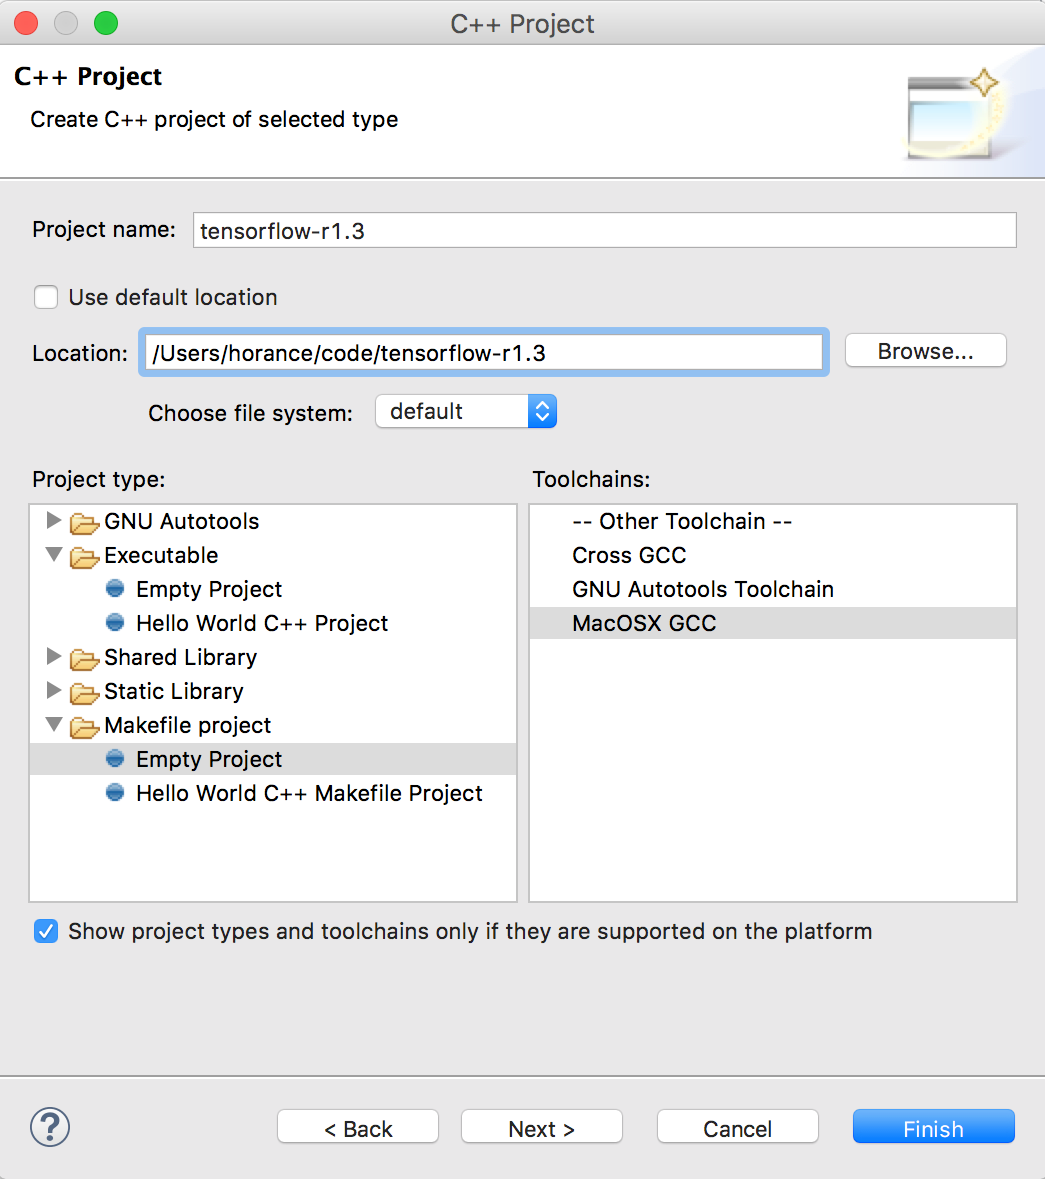
\includegraphics[width=0.75\textwidth]{figures/setup-eclipse.png}
\caption{创建Eclipse C++工程}}
 \label{fig:setup-eclipse}
\end{figure}

\subsubsection{配置Eigen}

不幸的是,\ascii{Eigen}对外公开的头文件缺少\code{.h}的后缀名,\ascii{CDT}无法解析相关的符号。请参阅\code{\href{http://eigen.tuxfamily.org/index.php?title=IDEs}{http://eigen.tuxfamily.org/index.php?title=IDEs}}相关说明,按照\ascii{Preferences > C/C++ > Coding Style > Organize Includes > Header Substitution}导入\code{eigen-header-substitution.xml}文件,如\refig{eclipse-eigen3}所示。

\begin{figure}[!htbl]
\centering
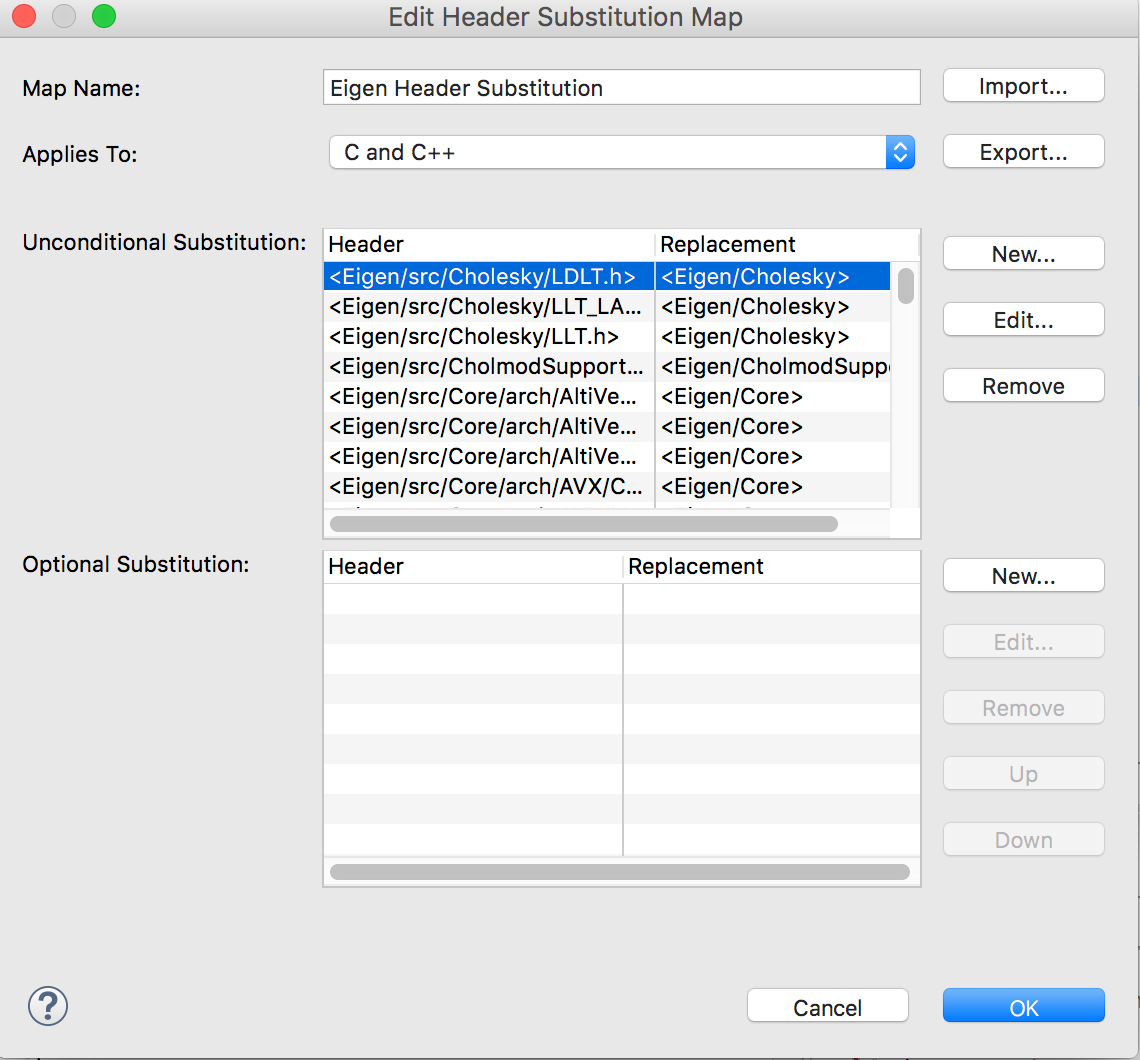
\includegraphics[width=0.75\textwidth]{figures/eclipse-eigen3.png}
\caption{替换\ascii{Eigen}的头文件}
 \label{fig:eclipse-eigen3}
\end{figure}

\end{content}

\section{代码生成}

\begin{content}

在构建\ascii{TensorFlow}系统时,\ascii{Bazel}或\ascii{CMake}会自动生成部分源代码。理解代码生成器的输出结果,可以加深理解系统的行为模式。

\end{content}

\section{技术栈}

\begin{content}

如\refig{tf-stack}所示,按照系统的层次结构展示了\tf{}的技术栈,构成了\tf{}生态系统的核心。

\begin{figure}[H]
\centering
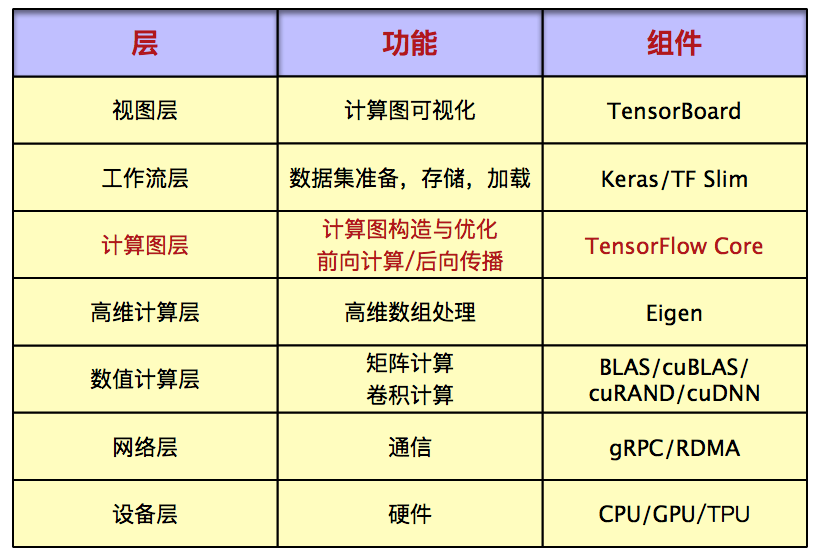
\includegraphics[width=0.7\textwidth]{figures/tf-stack.png}
\caption{TensorFlow技术栈}}
 \label{fig:tf-stack}
\end{figure}

\end{content}
